 \documentclass[oneside,a4paper,12pt]{book}
%\pagestyle{headings}
\frontmatter

%=============================================================================

\usepackage{amsthm}
\usepackage{xspace}
\usepackage{float}
\usepackage{ifthen}
\usepackage{amsbsy}
\usepackage{amssymb}
\usepackage{balance}
\usepackage{booktabs}
\usepackage{graphicx}
\usepackage{rotating}
\usepackage{multirow}
\usepackage{needspace}
\usepackage{microtype}
\usepackage{bold-extra}
\usepackage{geometry}
\usepackage{varioref}
\usepackage{xcolor}
\usepackage{textcomp}
\usepackage{listings}
\usepackage[normalem]{ulem} %emphasize still italic
\usepackage{ucs}

% \usepackage[utf8]{inputenc}
% \usepackage[htt]{hyphenat}
\usepackage{times}
\usepackage{url}
\usepackage{alltt}
\usepackage{amsmath}
\usepackage{xfrac}
\usepackage{subfigure}
\usepackage{appendix}
\usepackage{stmaryrd}   % for the \shortuparrow
\usepackage[utopia]{quotchap}

\usepackage{setspace}
\usepackage[numbers, sort&compress]{natbib}
\usepackage{mdwlist}        % support for better spaced lists
% allows for temporary adjustment of side margins
\usepackage{chngpage}
\usepackage[normalem]{ulem} 

% lina entered
\usepackage{indentfirst}
\usepackage[parfill]{parskip}
\usepackage[bottom]{footmisc}

\usepackage[T1]{fontenc}
\usepackage{caption}
\usepackage{booktabs}
\usepackage{siunitx}


\setlength{\parindent}{1.5em}

% constants

\newcounter{qcounter}

% commands
\newcommand{\n}{$\cdot$}
\newcommand{\y}{\checkmark}
\newcommand{\subscript}[1]{$_{\textrm{\footnotesize{#1}}}$}
\newcommand{\superscript}[1]{$^{\textrm{\footnotesize{#1}}}$}
\newcommand{\vertical}[1]{\raisebox{-4em}{\begin{sideways}{#1}\end{sideways}}}
\newcommand\tab[1][1cm]{\hspace*{#1}}

\usepackage{boxedminipage}

\newboolean{showedits}
\setboolean{showedits}{true} % toggle to show or hide edits
\ifthenelse{\boolean{showedits}}
{
       \newcommand{\ugh}[1]{\textcolor{red}{\uwave{#1}}} % please rephrase
       \newcommand{\ins}[1]{\textcolor{blue}{\uline{#1}}} % please insert
       \newcommand{\del}[1]{\textcolor{red}{\sout{#1}}} % please delete
       \newcommand{\chg}[2]{\textcolor{red}{\sout{#1}}{\ra}\textcolor{blue}{\uline{#2}}} % please change
}{
       \newcommand{\ugh}[1]{#1} % please rephrase
       \newcommand{\ins}[1]{#1} % please insert
       \newcommand{\del}[1]{} % please delete
       \newcommand{\chg}[2]{#2}
}


% ============================================================================
% Put edit comments in a really ugly standout display

\usepackage{xcolor}
\usepackage[normalem]{ulem}
\newcommand{\ra}{$\rightarrow$}
\usepackage{amssymb}

% comments \nb{label}{color}{text}
\newboolean{showcomments}
\setboolean{showcomments}{true}
%\setboolean{showcomments}{false}
\ifthenelse{\boolean{showcomments}}
{\newcommand{\nb}[3]{
  {\colorbox{#2}{\bfseries\sffamily\scriptsize\textcolor{white}{#1}}}
  {\textcolor{#2}{\sf\small$\blacktriangleright$\textit{#3}$\blacktriangleleft$}}}
    \newcommand{\version}{\emph{\scriptsize$-$Id$-$}}
%	 \newcommand{\ugh}[1]{\textcolor{red}{\uwave{#1}}} % please rephrase
%	 \newcommand{\ins}[1]{\textcolor{blue}{\uline{#1}}} % please insert
%	 \newcommand{\del}[1]{\textcolor{red}{\sout{#1}}} % please delete
%	 \newcommand{\chg}[2]{\textcolor{red}{\sout{#1}}{\ra}\textcolor{blue}{\uline{#2}}} % please change
	 \newcommand{\chk}[1]{\textcolor{ForestGreen}{#1}} % changed, please check
	}
{\newcommand{\nb}[3]{}
  \newcommand{\version}{}
  \newcommand{\chk}[1]{} % changed, please check
  }
\newcommand\nm[1]{\nb{NM}{violet}{#1}} % add more author macros here
\newcommand\lt[1]{\nb{LT}{orange}{#1}}


% ============================================================================
% Make quotes be italic
\renewenvironment{quote}
    {\list{}{\rightmargin\leftmargin}%
     \item\relax\begin{it}}
    {\end{it}\endlist}

\newcommand{\ttimes}{\ensuremath{\times}}

%=============================================================================

\newcommand{\needlines}[1]{\Needspace{#1\baselineskip}}

% source code
\usepackage{xcolor}
\usepackage{textcomp}
\usepackage{listings}
\definecolor{javared}{rgb}{0.6,0,0} % for strings
\definecolor{javagreen}{rgb}{0.25,0.5,0.35} % comments
\definecolor{javapurple}{rgb}{0.5,0,0.35} % keywords
\definecolor{javadocblue}{rgb}{0.25,0.35,0.75} % javadoc

\renewcommand{\lstlistingname}{Code}% Listing -> Algorithm
\renewcommand{\lstlistlistingname}{List of \lstlistingname s}% List of Listings -> List of Algorithms

\lstnewenvironment{Java}[1][]
{\lstset{
	language=Java,
	basicstyle=\footnotesize\ttfamily,
	keywordstyle=\color{javapurple}\bfseries,
	stringstyle=\color{javared},
	commentstyle=\color{javagreen},
	morecomment=[s][\color{javadocblue}]{/**}{*/},
	numbers=left,
	numberstyle=\tiny\color{black},
	stepnumber=1,
	numbersep=10pt,
	tabsize=4,
	showspaces=false,
	showstringspaces=false,
	breaklines=true,
	captionpos=b,
	xleftmargin=2em,
	framexleftmargin=1.5em,
	frame=single,
	#1
}}
{}


\lstnewenvironment{JVMIS}[1][]
{\lstset{
	language=JVMIS,
	basicstyle=\footnotesize\ttfamily,
	keywordstyle=\color{javagreen}\bfseries,
	stringstyle=\color{javared},
	commentstyle=\color{javagreen},
	morecomment=[s][\color{javadocblue}]{/**}{*/},
	numbers=none,
	numberstyle=\tiny\color{black},
	stepnumber=1,
	numbersep=10pt,
	tabsize=4,
	showspaces=false,
	showstringspaces=false
	breaklines=true,
	captionpos=b,
	xleftmargin=2em,
	framexleftmargin=1.5em,
	frame=single,
	#1
}}
{}


\definecolor{codegray}{gray}{0.9}
\newcommand{\code}[1]{
	\colorbox{codegray}
	{\texttt{#1}}
}

%----------------------------------------------------------------------------
% references
\newcommand{\tabref}[1]{\hyperref[{tab:#1}]{Table~\ref*{tab:#1}}}
\newcommand{\figref}[1]{\hyperref[{fig:#1}]{Figure~\ref*{fig:#1}}}
\newcommand{\secref}[1]{\hyperref[{sec:#1}]{Section~\ref*{sec:#1}}}
\newcommand{\subsecref}[1]{\hyperref[{subsec:#1}]{Subsection~\ref*{subsec:#1}}}
\newcommand{\lstref}[1]{\hyperref[{lst:#1}]{Listing~\ref*{lst:#1}}}
\newcommand{\charef}[1]{\hyperref[{ch:#1}]{Chapter~\ref*{ch:#1}}}
\newcommand{\coderef}[1]{\hyperref[{code:#1}]{Code~\ref*{code:#1}}}
\newcommand{\bytecoderef}[1]{\hyperref[{bytecode:#1}]{Bytecode~\ref*{bytecode:#1}}}
\newcommand{\algref}[1]{\hyperref[{alg:#1}]{Algorithm~\ref*{alg:#1}}}
\newcommand{\boxref}[1]{\hyperref[{box:#1}]{Box~\ref*{box:#1}}}

%----------------------------------------------------------------------------

% abbreviations
\tracingcolors 4
\setcounter{tocdepth}{3}
\setcounter{secnumdepth}{3}
\newcommand{\ie}{\emph{i.e.,}\xspace}
\newcommand{\eg}{\emph{e.g.,}\xspace}
\newcommand{\etc}{\emph{etc.}\xspace}
\newcommand{\etal}{\emph{et al.}\xspace}


\newcommand{\newevenside}{
	\ifthenelse{\isodd{\thepage}}{\newpage}{
	\newpage
        \phantom{placeholder} % doesn't appear on page
	\thispagestyle{empty} % if want no header/footer
	\newpage
	}
}

\def\stretchfactor{1}
\newcommand{\mychapter}[1]{\setstretch{1}
    \chapter{#1}\setstretch{\stretchfactor}}

%----------------------------------------------------------------------------
\newcommand{\lessSpace}{\vspace{-1em}}
\DeclareGraphicsExtensions{.pdf,.png}
\graphicspath{{images/}}
\newcommand{\fig}[4]{
	\begin{figure}[#1]
		\centering
		\includegraphics[width=#2\textwidth]{#3}
		\lessSpace
		\caption{\label{fig:#3}#4}
	\end{figure}}

% ===========================================================================

%:CONFIGURE THIS

\newcommand{\thesistitle}{Where does this null come from ?}
\newcommand{\thesisauthor}{Lina Tran}
\newcommand{\thesisauthorOrigin}{Biel/Bienne BE, Switzerland}
\newcommand{\thesisleiter}{Prof.\ Dr.\ Oscar Nierstrasz}
\newcommand{\thesisasst}{	\begin{center}
														Research assistant Nevena Milojkovi\'{c}\\
														Research assistant Boris Spasojevi\'{c}
													\end{center}}
\newcommand{\thesisurl}{http://scg.unibe.ch/}
\newcommand{\thesissubtitle}{An Approach to show the exact location where a value was referenced to null}
\newcommand{\thesisdate}{31. July 2016}

% ===========================================================================

\usepackage[ colorlinks=true, urlcolor=black, linkcolor=black,
			citecolor=black, bookmarksnumbered=true, bookmarks=true,
			plainpages=false,
			pdftitle={\thesistitle}, pdfauthor={\thesisauthor},
			pdfsubject={\thesissubtitle}, pdfpagelabels]{hyperref}

\newcommand{\hrref}[2]{\hyperref}
% ===========================================================================
% ===========================================================================


% D O C U M E N T
% % % % % % % % % % % % % % % % % % % % % % % % % % % % % % % % % %
\begin{document}

% T I T L E
% % % % % % % % % % % % % % % % % % % % % % % % % % % % % % % % % %
\begin{titlepage}  
  \begin{center}  
  
  \begin{figure}[t]  
  \vspace*{-2cm}        % to move header logo at the top 
  \center{
\includegraphics[scale=0.5]{logos/UNI_Bern.png}}
  \vspace{1in}     
  \end{figure}

    \thispagestyle{empty}
    
    {\bfseries\Huge \thesistitle \par
    \Large \vspace{0.1in} \thesissubtitle \par}

    \vspace{0.3in} 
    \LARGE{\textbf{Bachelor Thesis} \\}
    \vspace{0.4in}

    {\Large \thesisauthor \par from \par \thesisauthorOrigin}
    
    \vspace{0.3in}
    {\Large Faculty of Science \\
            University of Bern \par}
    \vspace{0.3in}
    {\Large \thesisdate \par}
    \vspace{0.3in}
    %Leiter der Arbeit: \par
   {\Large \thesisleiter} \par
      {\Large \thesisasst} \par
   \vspace{0.1in}
    {\Large Software Composition Group \par Institute for Computer Science \par University of Bern, Switzerland \par}
  

  %\vspace{0.5in}
 
 

  \end{center}

\end{titlepage}


% A B S T R A C T
% % % % % % % % % % % % % % % % % % % % % % % % % % % % % % % % % %
\chapter*{\centering Abstract}
\begin{quotation}
\noindent 
A previous study found out that NullPointerExceptions are very serious in Java projects. When a NullPointerExceptions occurs the developer is provided only with a stack trace to where the exception happened. This only gives insight into the effect of the fault but not into its cause. So we have to ask the question when and why this reference was set to null.

The aim of the project is to be able to provide the user with an additional stack trace of where the value was actually set to null, next to the normal stack trace of an exception. We attempt to achieve this goal by instrumenting java source code ideally with a minimal overhead. 

By tracking the null assignments the debugging after a NullPointerException will be simplified. 
\end{quotation}
\clearpage


% C O N T E N T S 
% % % % % % % % % % % % % % % % % % % % % % % % % % % % % % % % % % % % % % % %
\tableofcontents

\mainmatter
%%%%%%%%%%%%%%%%%%%%%%%%%%%%%%%%%%
%%%% NEW CHAPTER %%%%%%%%%%%%%%%%%%%%%
%%%%%%%%%%%%%%%%%%%%%%%%%%%%%%%%%%
\chapter{Introduction}
\label{ch:introduction}
Nowadays, certainly every programmer is confronted with NullPointerExceptions in big Java Projects, whether it is for an enterprise or for private purposes. Not to mention even in small Java Projects they are also heavily present.

So what are those NullPointerExceptions? This thesis is going to attach importance to Java that is a concurrent, class-based, object-oriented programming language. We chose Java because NullPointerExceptions are more serious in this language than in others, e.g. Smalltalk. NullPointerException is a RuntimeException. In Java, an object reference can be assigned with a special null value. The exception is thrown when an application attempts to use an object reference that has the null value. (There are multiple ways this exception can be thrown, like: Calling an instance method on the object referred by a null reference; Accessing or modifying an instance field of the object referred by a null reference and so on.) In Java Projects developers always have to deal with a huge amount of references which means avoiding these NullPointerExceptions is as good as impossible.

On regular meetings among programmers they report what they have been doing and what they are planning to do for the next few weeks. But all too often it is stated that they are trying to fix bugs or have spent a lot of time fixing them. If there would be a way to minimize the time fixing exceptions and allow to work more efficiently, projects would progress much faster.

The main goal of the NullSpy application takes a step to that ideal vision. Anytime developers are facing a NullPointerException they don’t have to spent time on debugging finding where and why a reference was set to null. With NullSpy the exact location of the null assignment is shown next to the ordinary stack trace the Java virtual machine produces.

In this thesis it is explained how the goal mentioned above is achieved step by step, by using a class library Javassist (Java Programming Assistant) which allows us to deal with Java bytecode.

\chapter {Technical Background}
\label{ch:technicalBackground}

This chapter provides a short overview of works/technologies used in this project.

\section{Javassist}
\label{sec:javassist}
Javassist or Java Programming Assistant\footnote{\url{http://jboss-javassist.github.io/javassist/}}, a subproject of Jboss, is a class library which allows you to deal with Java bytecode. Since 1999 it is used as an engineering toolkit in a broad domain, and is still being extended by Shigeru Chiba. It enables developers to manipulate Java bytecode in a simplified way like defining a new class at runtime or modifying a class file when it is loaded by the JVM. All manipulations are performed at load-time through a provided class loader.

\begin{figure}[H]
\centering
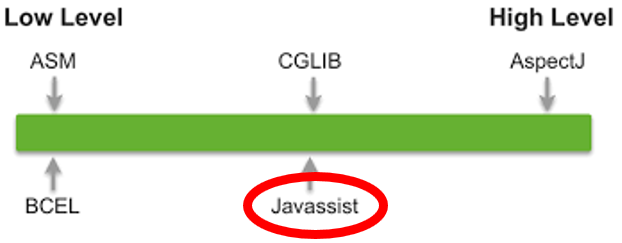
\includegraphics[width=0.8\linewidth]{bytecodeModificationLevels}
\caption{Bytecode modification levels}
  \label{fig:bytecodeModificationLevels}
\end{figure}

Unlike many other libraries Javassist offers two levels of API: source level and bytecode level (See figure \ref{fig:bytecodeModificationLevels}). Using the source-level API, the user can edit a class file without any familiarity with the specifications of the Java bytecode. Only knowing the Java language is enough because the API is designed only with the vocabulary of Java. On this level the programmer just has to write normal source code and Javassist compiles it automatically. The bytecode level allows the user to modify classes directly in binary form like other editors, e.g. ASM.

At this point, let us look at a small example to give you an idea how the bytecode manipulation works.

\begin{figure}[H]
\centering
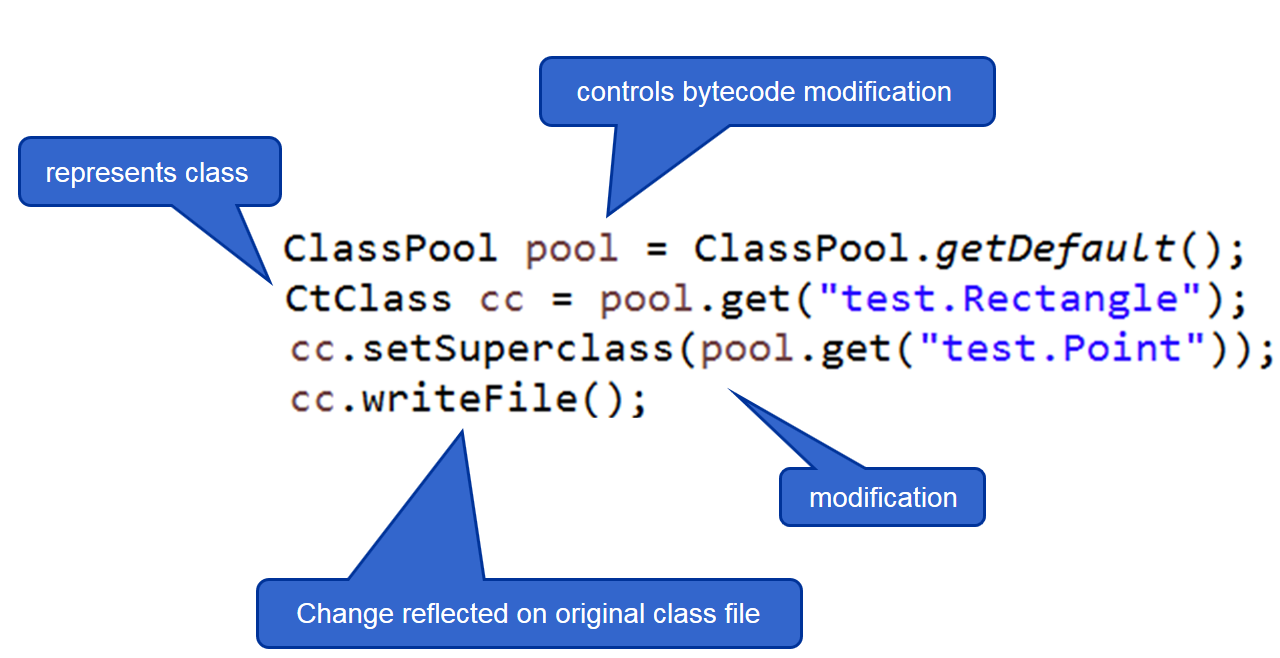
\includegraphics[width=0.8\linewidth]{javassistExample}
\caption{Javassist example}
  \label{fig:javassistExample}
\end{figure}

First a ClassPool object is obtained that controls bytecode modification with Javassist. With the ClassPool a class file can be read on demand for constructing a CtClass object. The class CtClass (compile-time class) is just an abstract representation of a class file which means all manipulations are performed on the CtClass. With the method invocation \textit{get()} on ClassPoola reference to the class file \textit{test.Rectangle} is obtained. In this example the superclass of \textit{test.Rectangle} is just changed to \textit{test.Point}. If the changes are done, the method call \textit{writeFile()} on CtClass is necessary to make sure that the changes are reflected on the original class file.\footnote{Getting started with Javassist: \url{http://jboss-javassist.github.io/javassist/tutorial/tutorial.html}}

\begin{figure}[H]
\centering
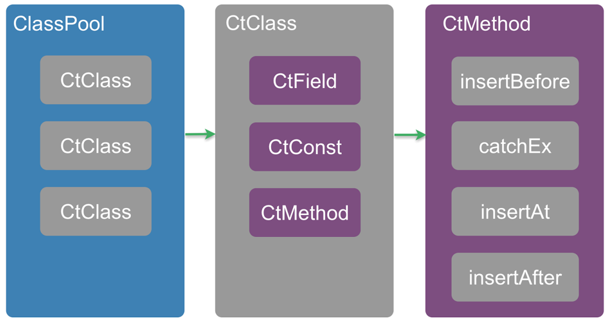
\includegraphics[width=0.8\linewidth]{javassistModules}
\caption{Javassist Modules}
  \label{fig:javassistModules}
\end{figure}

Figure \ref{fig:javassistModules} gives you an understanding/overview how the main part of bytecode manipulation with Javassist is built up. The ClassPool is nothing else than a container of multiple CtClasses. As described before CtClass is just the abstract representation of a class file on which modifications are done. Like typical classes, it can hold several compile-time fields, constants or methods. While speaking about bytecode manipulation all the time, nothing but editing methods is manly meant. It is possible to insert additional source code at the beginning of the method body, at the end or at a specific line. Next to these options even a \textit{catchBlock} can be added.

\begin{figure}[H]
\centering
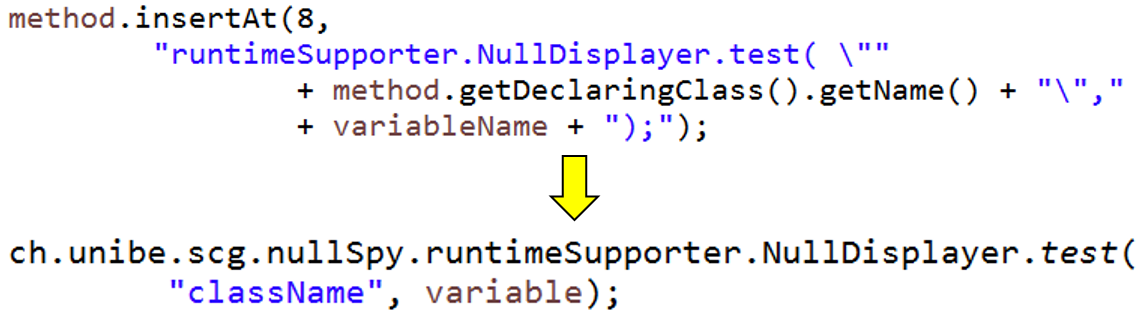
\includegraphics[width=0.9\linewidth]{insertionCodeExample}
\caption{Inserting code example}
  \label{fig:insertionCodeExample}
\end{figure}

\section{JAD}
JAva Decompiler\footnote{\url{https://sourceforge.net/projects/jadclipse/}} is a decompiler and a Eclipse plugin for the programming language Java. A short explanation what a decompiler is: a computer program that takes an executable file as input, and attempts to create a high level, compatible source file that does the same thing. So it is used in software reverse engineering.

\begin{figure}[H]
\centering
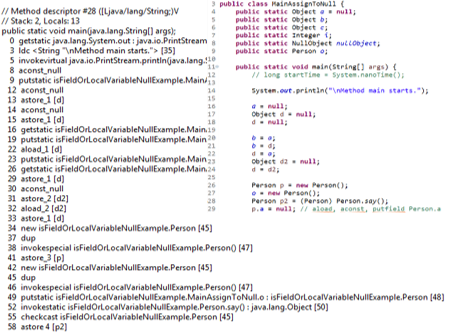
\includegraphics[width=0.6\linewidth]{bytecodeSourcecode}
\caption{Decompile example}
  \label{fig:bytecodeSourcecode}
\end{figure}

JAD is used in NullSpy since after running NullSpy on a project only the modificated bytecodes are available. To simplify the check whether the modification by Javassist, e.g. inserting source code, has succeeded, a decompiler is needed.

\chapter{NullSpy}
As earlier explained in the introduction (\ref{ch:introduction}), this project is about providing the user with additional stack trace where the origin of a NullPointerException is actually rooted. Briefly worded, it shows the developer the exact location of where a method receiver, which causes the NPE, was assigned to null.

This is the main chapter of the thesis. Here we would like to give you a short insight of how we managed to successfully implement the core of the project NullSpy. Next to how it is built up, we will also let you know what challenges we were encountering during the implementation and about the limitations we planned for future work (\ref{ch:conclusionsFutureWork}).


\section{High level overview/Rough Scheme}
The general approach of NullSpy is to statically analyze and add additional bytecode to a project. After reading the section Javassist (\ref{sec:javassist}) you should be more familiar with how bytecode manipulation with Javassist works.

What NullSpy first does is loading the project you want it to be able to track the null assignment if a NullPointerException is thrown. By loading the project to NullSpy, the compiled class files of the project are addressed only, which means the project itself does not have to be imported to the programming environment, e.g. Eclipse. Simultaneously at load time each class file is modified with help of Javassist; In what way will be discussed in the following section “Low level overview”.

Once the project modification is done it is stored in a destination folder that the user has chosen before. This means after the changes there will be another version of the project which can do additional stuff like tracking the null assignment. Because only the class files are accessed previously, the result which is stored in the destination folder is as expected only the modified bytecode.

How do we check whether the instrumentation worked and the project really tracks the null assignment? The answer is wrapping the modified project into a jar file with which the modified project can be executed in the terminal or in Eclipse.

\begin{figure}[H]
\centering
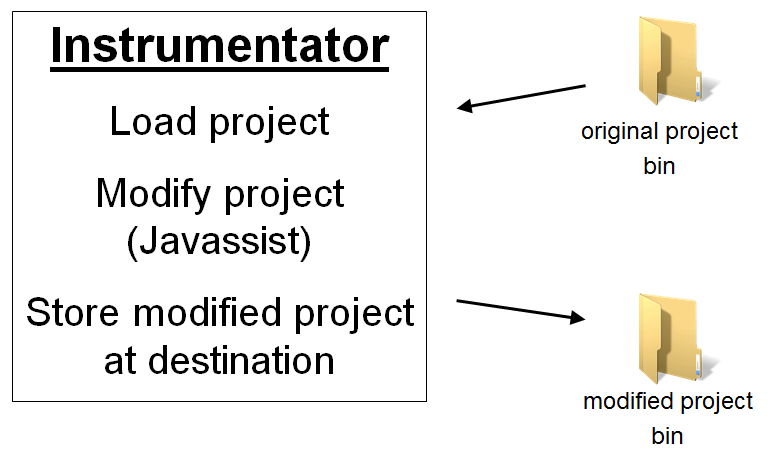
\includegraphics[width=0.5\linewidth]{highLevelOverview}
\caption{Modification overview}
  \label{fig:highLevelOverview}
\end{figure}


\section{Low level overview}
So we first load the project which should be modified and then go through all class files of it. A NullPointerException can only be thrown if a method call was performed on a method receiver which is null. That means we have to gather information about the method receiver. To know the exact location of the null assignment of course we also have to collect information about the variable assignments.

The main idea behind NullSpy actually is to get information about method receivers and information about the variables on one side and comparing those together if a NullPointerException occurs on the other side. If there is a hit on the matching the null assignment location can be obtained easily.

\subsection{Method Receiver Data Collection}
\label{subsec:methodReceiver}
Unfortunately, Javassist does not provide the function to directly get the method receiver. We got a suggestion to use AST (Abstract Syntax Tree footnote wiki) to get it but we decided to not go deeper into this and implement our own algorithm.

The algorithm contains following steps (abstract):\newline\newline
\fbox{
\begin{minipage}{\linewidth}
\begin{enumerate}
\itemsep8pt
      \item Getting pc-interval of method invocation
      \item Storing all possible method receiver interval within the interval of step 1 into an ArrayList
			\item Getting the number of parameters, the method invocation takes
			\item Traversing back the ArrayList the amount of parameters obtained in step 3
			\item Result: method receiver interval
			\item Store variable name, type etc. into an external csv file
   \end{enumerate}
	\end{minipage}
	}
\newline\newline\newline
In step 1 we had big troubles getting the right interval of the method receiver because only by statically analyzing the bytecode it is unapparent where the method receiver is situated exactly. But more about the challenges you will learn more in chapter \ref{subsec:methodReceiverTroubles}.

Statically analyzing bytecode for method receiver means looking for certain opcodes which matches all opcodes that matches with the regex \textit{''invoke.*''}}. There are exactly five kinds of bytecode instruction: \textit{invokedynamic}, \textit{invokeinterface}, \textit{invokespecial}, \textit{invokestatic}, \textit{invokevirtual}. The invocation opcode invokedynamic facilitates the dynamic-typed languages\footnote{Language whose type checking is usually performed at runtime.} through dynamic method invocation. In our case it can be ignored because NullSpy only supports the static-typed language\footnote{Language whose type checking is performed at compile time.} Java.

In case of the \textit{invokestatic} instruction we do not have a method receiver. That is why NullSpy treats it extraordinary like ignoring it completely or wrap it as a possible method receiver when it is actually a parameter of a method invocation. In all other cases we normally use the algorithm to get the method receiver.

\subsection{Variable Data Collection}
\label{subsec:variable}
While going through the bytecode attention is paid to some opcodes\footnote{Operation code: Machine language instruction.}. Right after each keyword that indicates a variable assignment we insert some bytecode. The inserted code represents a test method which tests whether the value of the assigned variable is null or not and store some information about it. Unlike in getting information about the method receiver in subsetion \ref{subsec:methodReceiver} the data about the variables are stored in a HashMap.

What kind of opcodes were NullSpy looking for? For instance or class/static variables the bytecode instruction \textit{getfield} and \textit{getstatic} were essential, for local variables the important opcodes were those which matches the regex \textit{''aload.*''}. Due to different types of variables and the limitation of Javassist gathering information about them was performed differently. Again getting the necessary data about the variables we encountered many difficulties which will be discussed in the subsection \ref{sec:challenges}.

Unfortunately, Javassist does not provide any support for gaining information about local variables that is why getting the needed data we had to understand how bytecode is constructed. At this point we would like to give you a small bytecode introduction.

\begin{figure}[H]
\centering
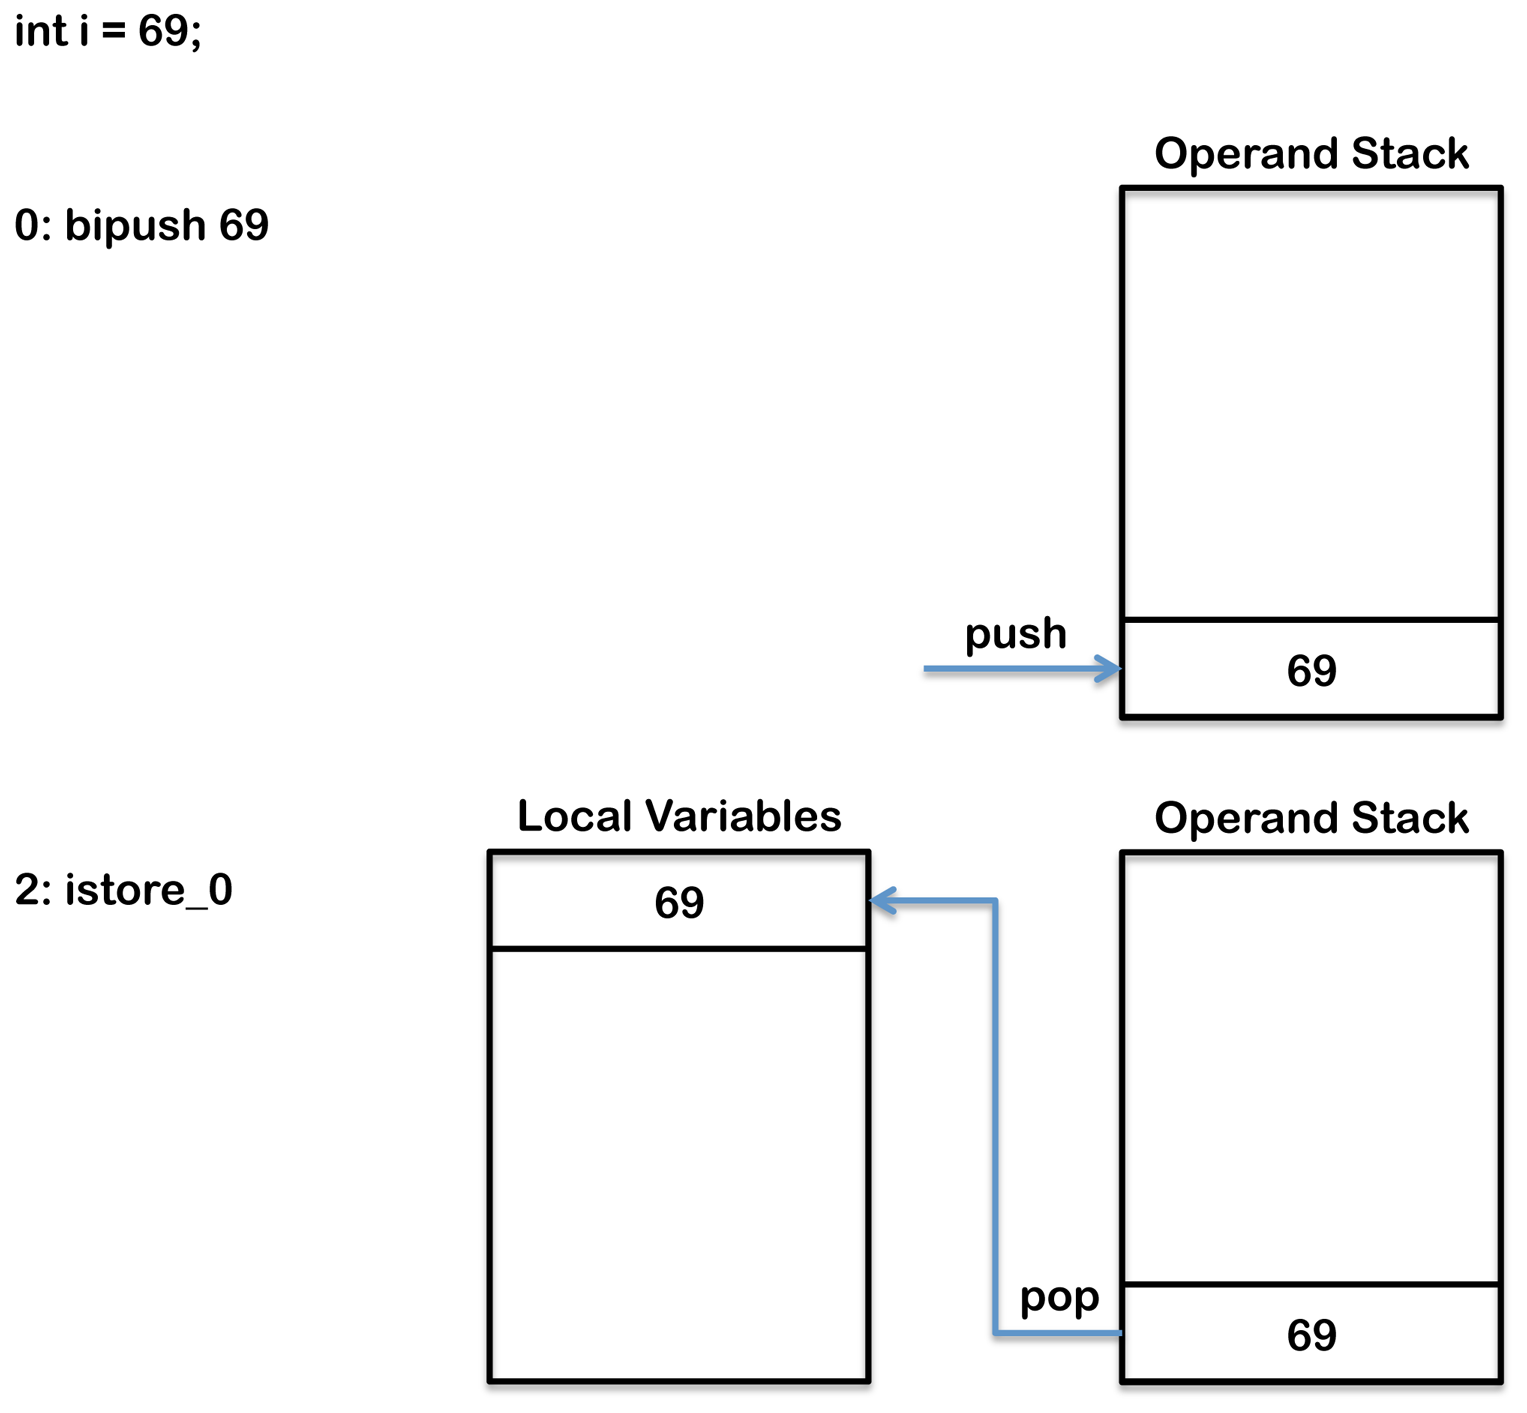
\includegraphics[width=0.5\linewidth]{localVarCreationBytecode}
\caption{Local variable creation bytecode\footnote{\url{http://blog.jamesdbloom.com/images_2013_11_17_17_56/java_local_variable_creation_byte_code.png}}}
  \label{fig:localVarCreationBytecode}
\end{figure}

If a local variable is created, the value assigned to it is pushed onto the operand stack. With the bytecode instruction \textit{''.*store.*''} the local variable is popped from the operand stack and stored into a local variable array slot. In which slot it is stored can be extracted from the instruction. Opcodes for storing local variables is composed of one, or in some cases two bytes. There are reserved machine commands for the first four local variables, index-linked from 0 to 3 and each of them contains one byte (astore\_0, astore\_1, astore\_2, astore\_3). If there is no slot number visible in the instruction, it indicates that the slot number is stored in the second byte from where it can be extracted. Next to storing the local variable loading it from the local variable array is possible to, but only with the local variable slot number.

With this short introduction understanding the local variable table should be easier. Each method of a class file contains a local variable table (see figure \ref{fig:localVarTable}) with which many information can be read out of it, e.g. the lifespan of the local variable, what it is called, in which slot it is stored and what type it has.

\begin{figure}[H]
\centering
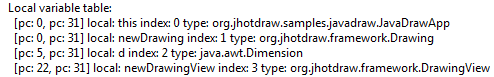
\includegraphics[width=\linewidth]{localVarTable}
\caption{Local variable table}
  \label{fig:localVarTable}
\end{figure}

We had to pay attention to be sure to get the right local variable. Every time when we bumped into the opcode ''.*store.*'' we could only get its slot and the pc\footnote{Program counter/instruction pointer: A processor register that indicates where a computer is in its program sequence.} where it is situated in the bytecode sequence. In the earlier paragraph the lifespan of the local variable was mentioned, the importance behind this is as soon as the lifespan of one ends, the slot can be reused by the next instantiated local variable. This way, the local variable table could contain multiple entries with the same local variable slot.

\begin{figure}[H]
\centering
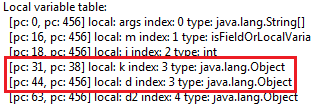
\includegraphics[width=0.7\linewidth]{localVarTableDuplicatedSlot}
\caption{Local variable table entries with same slot}
  \label{fig:localVarTableDuplicatedSlot}
\end{figure}

After extracting the slot of the local variable we will get the first local variable table entry which contains that slot. If the pc of the local variable assignment is not included in the lifespan-pc-interval of the entry, the next entry with the same slot will be checked until both criteria (slot and pc) fits. Once those criteria are met we can be positive about having got the right local variable table entry to extract the information needed.

Next to the local variable table each methods of a class file also holds another attribute called line number attribute. This is just the mapping table from pc to source code line number. Since encountering the storing keyword the pc is available , with help of it the line number can be easily obtained.

\begin{figure}[H]
\centering
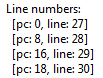
\includegraphics[width=0.3\linewidth]{lineNrTable}
\caption{Line number table}
  \label{fig:lineNrTable}
\end{figure}

There was a big problem about inserting additional source code after assignments in certain situations. It is mainly caused by the limitation of the class library Javassist (see \ref{subsec:variableTroubles}).


\section{Challenges}
\label{sec:challenges}
..

\subsection{Obtaining Method Receiver Data Difficulties}
\label{subsec:methodReceiverTroubles}
bla bla

...

\subsection{Obtaining Variable Data Difficulties}
\label{subsec:variableTroubles}
bla bla

...
\section{Limitations}
...

\chapter{Validation}
In which you show how well the solution works.

\section{JHotDraw}
JHotDraw
To check whether the logic of the bytecode manipulation in this project NullSpy is working as desired, we had to perform them on a large working project. Thanks to Nevena Milojkovi\'{c} and her experience with the combination Javassist and JHotDraw we as well decided to test NullSpy on the project JHotDraw.
It is an open-source Java GUI framework for technical and structured Graphics. Its original authors have been Erich Gamma and Thomas Eggenschwiler. 

\chapter {Conclusion and Future Work}
\label{ch:conclusionsFutureWork}
In which we step back, have a critical look at the entire work, then conclude, and learn what lays beyond this thesis.

\chapter {Anleitung zu wissenschaftlichen Arbeiten}
This consists of additional documentation, e.g. a tutorial, user guide etc.
Required by the Informatik regulation.

%END Doc
%-------------------------------------------------------

\bibliography{thesis}
\bibliographystyle{plain}

\clearpage
\thispagestyle{empty}
\null\vfill
\begin{center}
''Ich erkl\"are hiermit, dass ich diese Arbeit selbstst\"andig verfasst und  keine  anderen  als  die  angegebenen  Quellen  benutzt  habe. 
Alle Stellen, die w\"ortlich oder sinngem\"ass aus Quellen entnommen  wurden,  habe  ich  als  solche  gekennzeichnet.  Mir  ist  bekannt,  dass  andernfalls  der  Senat  gem\"ass  Artikel 36  Absatz 1 Buchstabe 
r  des  Gesetzes  vom  5. September 1996  \"uber  die  Universit\"at zum Entzug des auf  Grund dieser Arbeit verliehenen Titels berechtigt ist.“
\vfill
\clearpage

\end{document}